\documentclass[12pt,a4paper]{article}
\usepackage[utf8]{inputenc}
\usepackage{amsmath}
\usepackage{amsfonts}
\usepackage{amssymb}
\usepackage{graphicx}
\usepackage[margin=2cm]{geometry}
\usepackage{subcaption}
\usepackage[french]{babel}


\usepackage{float}
\usepackage{notoccite}
\usepackage{url}



%title
\usepackage{titling}
\newcommand{\mytitle}{Projet : Multicores embarqué pour Big Data et
	Machine Learning}
\author{\textbf{DOU Yuhan\\ FORCIOLI Quentin \\ GHAOUI Mohamed Anis\\  TERRACHER Audrey}}

%header
\usepackage{fancyhdr}
\usepackage{lastpage}
\fancyhf{}
\lhead{\leftmark}
\rfoot{Page \thepage\ of \pageref{LastPage}}


%hypersetup
\usepackage{hyperref}
\hypersetup{
	colorlinks=true,
	linkcolor=black,
	filecolor=magenta,      
	urlcolor=black,
	pdftitle={\mytitle},
	pdfauthor=GHAOUI Mohamed Anis,
	pdfpagemode=Maximize,
	citecolor=black,
}

%listings
\usepackage{minted}

%figures
\usepackage{caption}
\usepackage{subcaption}



\begin{document}
\begin{titlepage}
\begin{center}
\vspace*{1cm}

\textbf{Master E3A}

\vspace{0.5cm}


Cours A2 : Systèmes Electroniques Embarqués

\vspace{1.5cm}
\mytitle

\vspace{1.5cm}
\theauthor

\vspace{1.5cm}
Encadré par :
\textbf{HAMMAMI Omar} et \textbf{LE PROVOST Hervé}
\vfill

Master 2 : Système Embarqué et Traitement de l'Information\\
\vspace{0.8cm}
Année : 2019-2020
\vspace{0.8cm}
\begin{center}
	
\includegraphics[width=0.4\textwidth]{logo}
	
\includegraphics[width=0.4\textwidth]{logo2}
\end{center}


\end{center}
\end{titlepage}

\newpage
%\tableofcontents
%\listoffigures
%\listoftables
\pagestyle{fancy}
\section{Introduction}


\section{Méthodologie et approche}
L'équipe consistant en 4 personnes, 2 personnes sont confiés la tâche de conception des logicielles à implémenter. i.e. Choisir les algorithmes à étudier, choisir le stratagème d'implémentation et la définition des besoins en terme de mécanisme C/C++, de jeu de données  et de tests à valider. Ensuite, Ils passent à une première implémentation qui n'est pas nécessairement optimisée afin de ne pas bloquer les autres parties de l'équipe. Une fois une première implémentation proposée au HLS, l'optimisation de cette implémentation pour ARM commence. Ce processus itératif consiste en l'analyse de l'architecture et contraintes de l'architecture cible comparée à l'architecture des ordinateurs usuels (PC bureau).

%parler de Spark et des algo
%%ajouter des trucs sur ça, mentioner les personnes?

La partie HLS consiste à analyser les implémentations C/C++ proposées par la partie logicielle embarquée, d'adapter ces implémentations d'algorithme aux contraintes matérielles sur la carte Zboard. En effet, certains mécanismes logiciels sont simplement impossibles à réaliser en matériel et donc la conception HLS sera une version modifiée afin de créer une IP implémentable et interfaçable dans un premier par ARM puis par $\mu$blaze.

\section{Conception logicielle embarquée}
%Quentin


% Parler du fait qu'on choisit d'implémenter la totalité dun algo ,  parole d'AUDREY
\section{Conception Synthèse Haut Niveau}
Cette conception dite HLS consiste à convertir un code C/C++ en une implémentation RTL d'un code VHDL ou Verilog. La difficulté de cette étape est de comprendre que tout ce qui est en C/C++ n'est pas forcement implémentable ou mal effectué par le trans-compilateur. En effet, on tente de passer d'un schéma de flot de contrôle vers un schéma de flot de données. Par exemple, le fonctions récursives sont simplement impossibles à implémenter matériellement. Certains algorithmes itératif à critères d'arrêt dynamique doivent subir une reconversion. Au final, le but est de générer une IP matérielle dite HLS et quelle soit implémentable par l'équipe gérant le matériel.

Dans cette partie, on présente le principe dernière l'outil HLS et quelques-unes des optimisations qu'il propose. Mais aussi, expliquera le raisonnement derrière l'approche de la génération matériellement automatisée.

\subsection{Conception d'une IP avec directives}
Une IP sera encapsulée en elle-même. Ce qui fait que l'implémentation matérielle n'aura aucun contrôle sur ce qui se passe dans l'IP.
Afin de pouvoir optimiser l'IP HLS créée, il faut dans un premier temps faire une analyse des dépendances pendant l'exécution de l'algorithme. Cette analyse est faite en 2 temps: 
\begin{itemize}
\item En premier, automatiquement par Vivado HLS qui possède des outils permettant de détecter des dépendances, d'essayer de les corriger/éliminer ou de suggérer à l'utilisateur d'utiliser les directives proposées.
\item En second, l'utilisateur, à l'aide des directives HLS, modifie la synthèse sans modifier le code lui même.
\end{itemize}
 Les directives les plus intéressantes, pour les algorithmes demandant plusieurs itérations et ayant une implémentation séquentielle tel que Kmeans, sont \texttt{FLATTEN}, \texttt{PIPELINE} et \texttt{UNROLL}.
 
\paragraph{Flatten} : Elle consiste à essayer de simplement aplatir la boucle en la rendant en une simple suite d'instructions. Ceci permettra de concevoir un flot de donnée matériel en RTL. Cette directive n'est possible que si toutes les boucles internes peuvent être aplaties et donc qu'il n'y ait pas de dépendances en données.
\paragraph{Pipeline} : Applicable aux boucles, fonctions et opérateurs, cette directive divise les opérations en plusieurs étages successifs de conception simple qui à chaque cycle effectuent une opération en 1 cycle. Le pipeline est très efficace pour diminuer la latence des opérateurs mais occupe une plus grande surface sur le FPGA contrairement à une version multi-cycles. Deux aspects important du pipeline sont : son intervalle d'initialisation (II) qui représente le nombre de cycles après lequel le pipeline peut consommer une donnée; et la latence i.e. le retard à la sortie.

\paragraph{Unroll} : Quand un calcul dans une boucle possède des dépendances de données et une latence plus grande que la durée d'une itération, il est conseillé de dérouler la boucle d'un facteur. par exemple au lieu de traiter les données 1 à 1, on peut traiter n à n. Cette directive peut occuper beaucoup plus de surface FPGA. Il faut donc l'utiliser uniquement quand le nombre d'itération est faible.

Une fois un opérateur/fonction optimisé(e), il faut analyser le nombre d'accès mémoire qu'il effectue en lecture/écriture. Si une mémoire ne fournit qu'un port d'accès, une seule lecture/écriture peut être fait en même temps dans le même cycle (en prenant en compte que la lecture prend deux cycles selon HLS). Il existe plusieurs stratagèmes pour contrer cela. HLS propose \footnote{\href{https://japan.xilinx.com/html\_docs/xilinx2017\_4/sdaccel\_doc/okr1504034364623.html}{Xilinx Pragma}} :
\paragraph{Map} : Permet d'agréger différents blocs mémoires en un seul afin de réduire l'usage des ressources RAM.
\paragraph{Partition} : Au contraire, cette directive permet de diviser un tableau en plusieurs sous tableau et donc blocs mémoires voir même registre afin d'augmenter le débit lecture/écriture au prix d'une coût matériel plus élevé.
\paragraph{Reshape} : Permet de redimensionner un bloc mémoire d'un certain facteur de manière entier ou cyclique afin d'avoir un bon compromis entre les deux directives précédentes. Celui-ci est le plus souvent utiliser car il permet d'avoir plusieurs accès mémoire matériels en fonction du nombre de circuits concurrents désirant d'accéder à la même donnée.

\subsection{Interfaçage d'une IP avec Axi/Axilite}
Il est possible d'interfacer une IP matériellement grâce à une panoplie de pointeurs bas niveau. Cette démarche permet d'avoir un contrôle très fin sur les adresses auxquelles le matériel accèdent. Mais par contre, complexifie tellement la gestion matérielle qu'elle devient très chronophage voir impossible pour un humain. Il est donc nécessaire de d'utiliser les interfaces fournis par Xilinx pour la carte ZedBoard, les \textit{Axi} et \textit{Axilite}. Il suffit de définir les ports entrées/sorties de l'IP HLS en tant que maître dans un port Axi et leur données une profondeur (la longueur de la mémoire FIFO). Aussi, il faut définir la fonction \textit{Top-level} comme étant apte à contrôler le bus et donc à recevoir les signaux de synchronisation depuis un CPU (soft ou hard) via l'interface \textit{Axilite}.

Dans les faits, On copie les entrées depuis l'interface du Axi dans des blocs mémoires locaux. Ceci fait que HLS infère des copies en rafale à la place de \textit{memcpy}.Donc, on travaille sur des pointeurs locaux puis on exporte le résultat par Axi output. Il ya donc une abstraction totale de l'interaction mémoire entre une IP HLS et le reste de l'architecture.

\subsection{Approche d'implémentation des algorithmes}
Afin de pourvoir transcrire les algorithmes discutés avec l'équipe logicielle, il d'abord effectuer une analyse de faisabilité en HLS. Car, on implémente pas un algorithme qui ne vaut pas le coût d'être accéléré. Ensuite, on procède à une analyse des besoins matériels pour en déduire les points d'apparition de goulots. Choisir entre la réinterprétation de l'algorithme ou la fragmentation en opérateurs.

Dans la première, on doit réétudier le processus de l'algorithme. Puis, décider si celui-ci est modifiable sans corrompre les résultats ou bien possède une autre implémentation qui puisse satisfaire au mieux les contraintes matérielles. Deux exemples : l'estimation du nombre $\pi$ par la méthode Monte-Carlo qui ne peut être effectué simplement car la fonction \texttt{rand()} n'existe pas en matériel. Il faut alors concevoir un générateur de nombre aléatoire matériel qu'il soit à base d'oscillateur en anneau ou autre. Un deuxième exemple est de modifier le critère d'arrêt de K-means i.e. changer la boucle \texttt{while} qui est d'une durée d'exécution indéterminé en boucle \texttt{for} qui elle est finie en terme de nombre d'itérations. Plusieurs autres optimisations sont faisables mais il n'y a pas de règles évidentes pour ceci. Il faut soit mener des recherches sur la documentation et les forums ou se fier à son intuition et expérience.

\subsubsection{Critères de conception d'IP}
Il existe un nombre assez élevé d'optimisation effectuées automatiquement ou manuellement par le logiciel HLS. Un premier facteur limitant lors de la conception est la surface FPGA occupée par l'IP (éléments logiques,DSP,...). Il est simplement impossible d'implémenter une IP qui ne peut pas être portée sur la carte. Donc, il faut limiter l'usage des directive \texttt{pipeline} et \texttt{unroll} mais aussi les blocs RAM internes.

Le deuxième paramètres limitant l'implémentation de l'IP est la fréquence de fonctionnement. HLS prend une période (donc fréquence) objective et "essayera" de synthétiser l'IP demandée à cette fréquence. Il est possible de le forcer à relaxer la synthèse afin de respecter ce critère.

Une solution possible à cette contrainte est d'utiliser des horloges différentes sur la carte qui ce soit par le Zynq ou le \texttt{SmartClock} (voir \ref{SmartClock}). La figure \ref{fig-hls} montre un résumé de quelques IPs implémentées. Toutes les IP ont pour période de fonctionnement objective : \textbf{10} ns.

\begin{figure}[H]
	\centering
	\begin{subfigure}[H]{.3\linewidth}
		\centering
		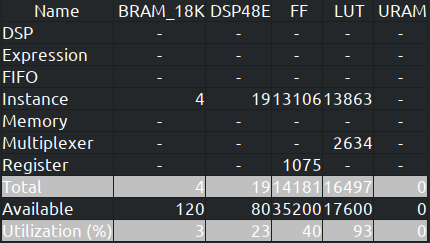
\includegraphics[width=\linewidth]{hls_fig/screenshot001}
		\caption{Peason}
	\end{subfigure}
	\begin{subfigure}[H]{.3\linewidth}
		\centering
		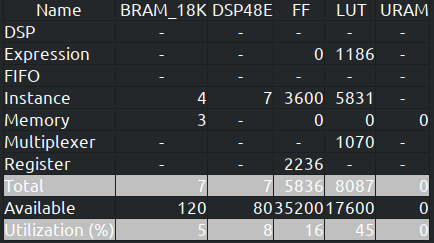
\includegraphics[width=\linewidth]{hls_fig/screenshot002}
		\caption{Kmeans}
	\end{subfigure}
	\begin{subfigure}[H]{.3\linewidth}
		\centering
		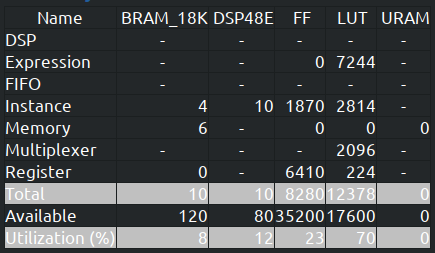
\includegraphics[width=\linewidth]{hls_fig/screenshot003}
		\caption{Matrix Block Mult.}
	\end{subfigure}	
	\caption{Occupation des ressources FPGA pour différentes IP}
	\label{fig-hls}
\end{figure}

\section{Implémentation matérielle}

% études des ports et connexions 

% instantiation micro blaze

% mémoire partagée problème et solution

% Implémentation de l'IP

\label{SmartClock}
Multi-horloge

\section{Conclusion}

\end{document}